\chapter{Orthogonal Matrices}

\section{预备知识}

\subsection{标准正交向量}

参见 \ref{Def:OrthonormalVectors}.

\subsection{Gram 矩阵与标准正交的关系}

For the definition of Gram matrices, refer to \ref{Def:Gram}. 关于它与非奇异的性质,参见 \ref{Sect:GramNonSingular}.

\begin{theorem}
    如果$A$的Gram矩阵为单位矩阵,则 $ A \in \mathbb{R}^{m \times n} $ 具有标准正交列。
\end{theorem}

\begin{proof}
    $$ \begin{aligned} A^{T} A&=\left[\begin{array}{llll}a_{1} & a_{2} & \cdots & a_{n}\end{array}\right]^{T}\left[\begin{array}{llll}a_{1} & a_{2} & \cdots & a_{n}\end{array}\right] 
    \\ &=\left[\begin{array}{cccc}a_{1}^{T} a_{1} & a_{1}^{T} a_{2} & \cdots & a_{1}{ }^{T} a_{n} \\ a_{2}^{T} a_{1} & a_{2}{ }^{T} a_{2} & \cdots & a_{2}^{T} a_{n} \\ \vdots & \vdots & \ddots & \vdots \\ a_{n}^{T} a_{1} & a_{n}^{T} a_{2} & \cdots & a_{n}^{T} a_{n}\end{array}\right] 
    \\  &=\left[\begin{array}{cccc}1 & 0 & \cdots & 0 \\ 0 & 1 & \cdots & 0 \\ \vdots & \vdots & \ddots & \vdots \\ 0 & 0 & \cdots & 1\end{array}\right] 
    \\ & =I  \end{aligned} $$
\end{proof}

\subsection{矩阵-向量乘积与标准正交的关系}

如果 $ A \in \mathbb{R}^{m \times n} $ 具有标准正交列,则线性函数 $ f(x)=A x $

\begin{theorem}
    保持原内积。
    $$ \langle A x, A y\rangle=x^{T} y $$
\end{theorem}

\begin{proof}
    $$ \langle A x, A y\rangle=(A x)^{T}(A y)=x^{T} A^{T} A y=x^{T} y $$
\end{proof}


\begin{theorem}
    保持原范数。
    $$
    \|A x\|_{2}=\|x\|_{2}
    $$
\end{theorem}

\begin{proof}
   $$
\|A x\|_{2}=\left((A x)^{T}(A x)\right)^{1 / 2}=\left(x^{T} x\right)^{1 / 2}=\|x\|_{2}
$$
\end{proof}

\begin{theorem}
    保持原距离。

    $$
    \|A x-A y\|_{2}=\|x-y\|_{2}
    $$
\end{theorem}

\begin{proof}
   $$
\|A x-A y\|_{2}=\left((A x-A y)^{T}(A x-A y)\right)^{1 / 2}=\left((x-y)^{T}(x-y)\right)^{1 / 2}=\|x-y\|_{2}
$$
\end{proof}

\begin{theorem}
    保持原角度。

    $$ \angle(A x, A y)=\angle(x, y) $$
\end{theorem}

\begin{proof}
    $$ \angle(A x, A y)=\arccos \left(\frac{(A x)^{T}(A y)}{\|A x\|_{2}\|A y\|_{2}}\right)=\arccos \left(\frac{x^{T} y}{\|x\|_{2}\|y\|_{2}}\right)=\angle(x, y) $$
\end{proof}

\subsection{左可逆性与正交的关系}


如果矩阵 $ A \in \mathbb{R}^{m \times n} $ 有标准正交列,则:

\begin{theorem}
    $ A $ 是左可逆的,其左逆为 $ A^{T} $.
\end{theorem}

\begin{proof}
    根据定义:

$$
A^{T} A=I
$$
\end{proof}

\begin{theorem}
    $ A $ 有线性无关的列向量。
\end{theorem}

\begin{proof}
    $$
A x=0 \quad \Rightarrow \quad A^{T} A x=x=0
$$
\end{proof}

\begin{theorem}
    $A$ 是高的或者方的, 即 $m \geq n$.
\end{theorem}

\begin{proof}
    列向量 $ a_{1}, a_{2}, \ldots, a_{n} \in \mathbb{R}^{m} $, 由维度定理可得 $ n \leq m $.
\end{proof}

\section{正交矩阵}

\begin{definition}[正交矩阵]
    所有列两两相互正交的\textbf{方形}实矩阵。
\end{definition}

\begin{theorem}[正交矩阵满足非奇异性]
    
    即如果矩阵 $ A $ 是正交的,则$ A $ 是可逆的,左逆等于右逆,且它的逆为 $ A^{T} $.

    $$ \left.\begin{array}{l}A^{T} A=I \\ A \text { 是方的 }\end{array}\right\} \quad \Rightarrow \quad A A^{T}=I $$
\end{theorem}

\begin{corollary}
    $ A^{T} $ 也是一个正交矩阵。
\end{corollary}

\begin{corollary}
    $ A $ 的行是标准正交的,即$a_i$范数为1且相互正交。
\end{corollary}

\begin{remark}
    如果 $ A \in \mathbb{R}^{m \times n} $ 有标准正交列以及 $ m>n $, 则 $ A A^{T} \neq I_{\text {. }} $
\end{remark}

\section{Permutation Matrices}

\begin{notation}
    $ \pi=\left(\pi_{1}, \pi_{2}, \ldots, \pi_{n}\right) $ 为 $ (1,2, \ldots, n) $ 的一个重新排序的排列。

    将 $ \pi $ 与一个置换矩阵 $ A \in \mathbb{R}^{n \times n} $ 联系起来:
$$
A_{i \pi_{i}}=1, \quad A_{i j}=0 \text { 如果 } j \neq \pi_{i}
$$
\end{notation}

\begin{definition}[置换]
    $ A x $ 是 $ x $ 的一个置换:
    
    $$ A x=\left(x_{\pi_{1}}, x_{\pi_{2}}, \ldots, x_{\pi_{n}}\right) $$
\end{definition}

$A$在每一行和每一列中都有一个等于1的元素。

\begin{theorem}
    置换矩阵满足正交性,即所有置换矩阵都是正交的。
\end{theorem}

\begin{corollary}
    $$ A^{T} A=I $$
\end{corollary}

\begin{proof}
    因为A的每一行有一个元素等于1
$$
\left(A^{T} A\right)_{i j}=\sum_{k=1}^{n} A_{k i} A_{k j}=\left\{\begin{array}{ll}
1 & i=j \\
0 & \text { 其它 }
\end{array}\right.
$$
\end{proof}

\begin{corollary}
    $ A^{T}=A^{-1} $是逆置换矩阵。
\end{corollary}

\begin{example}
    若 $ \{1,2,3,4\} $ 的置换为:
$$
\left(\pi_{1}, \pi_{2}, \pi_{3}, \pi_{4}\right)=(2,4,1,3)
$$

相应的置换矩阵及其逆矩阵为

$$ A=\left[\begin{array}{llll}0 & 1 & 0 & 0 \\ 0 & 0 & 0 & 1 \\ 1 & 0 & 0 & 0 \\ 0 & 0 & 1 & 0\end{array}\right] , A^{-1}=A^{T}=\left[\begin{array}{llll}0 & 0 & 1 & 0 \\ 1 & 0 & 0 & 0 \\ 0 & 0 & 0 & 1 \\ 0 & 1 & 0 & 0\end{array}\right] $$

$ A^{T} $ 是与置换相关的置换矩阵

$$
\left(\tilde{\pi}_{1}, \tilde{\pi}_{2}, \tilde{\pi}_{3}, \tilde{\pi}_{4}\right)=(3,1,4,2)
$$
\end{example}

\section{平面旋转}

\begin{FigureCenter}{An example of rotation}
    \tikzset{every picture/.style={line width=0.75pt}} %set default line width to 0.75pt        

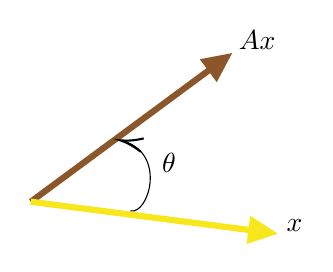
\begin{tikzpicture}[x=0.75pt,y=0.75pt,yscale=-1,xscale=1]
%uncomment if require: \path (0,300); %set diagram left start at 0, and has height of 300

%Straight Lines [id:da5121306887606891] 
\draw [color={rgb, 255:red, 139; green, 87; blue, 42 }  ,draw opacity=1 ][line width=2.25]    (100,112) -- (192.99,43.35) ;
\draw [shift={(197.01,40.38)}, rotate = 503.56] [fill={rgb, 255:red, 139; green, 87; blue, 42 }  ,fill opacity=1 ][line width=0.08]  [draw opacity=0] (14.29,-6.86) -- (0,0) -- (14.29,6.86) -- cycle    ;
%Straight Lines [id:da027572763792303556] 
\draw [color={rgb, 255:red, 248; green, 231; blue, 28 }  ,draw opacity=1 ][fill={rgb, 255:red, 248; green, 231; blue, 28 }  ,fill opacity=1 ][line width=2.25]    (100,112) -- (214.05,126.74) ;
\draw [shift={(219.01,127.38)}, rotate = 187.36] [fill={rgb, 255:red, 248; green, 231; blue, 28 }  ,fill opacity=1 ][line width=0.08]  [draw opacity=0] (14.29,-6.86) -- (0,0) -- (14.29,6.86) -- cycle    ;
%Curve Lines [id:da28950702982590015] 
\draw    (148.01,116.38) .. controls (156.78,118.33) and (165.56,88.91) .. (144.67,82.8) ;
\draw [shift={(143.01,82.38)}, rotate = 372.26] [color={rgb, 255:red, 0; green, 0; blue, 0 }  ][line width=0.75]    (10.93,-3.29) .. controls (6.95,-1.4) and (3.31,-0.3) .. (0,0) .. controls (3.31,0.3) and (6.95,1.4) .. (10.93,3.29)   ;

% Text Node
\draw (162,87.4) node [anchor=north west][inner sep=0.75pt]    {$\theta $};
% Text Node
\draw (222,119.4) node [anchor=north west][inner sep=0.75pt]    {$x$};
% Text Node
\draw (199,28.4) node [anchor=north west][inner sep=0.75pt]    {$Ax$};


\end{tikzpicture}
\end{FigureCenter}



\begin{example}[Rotation Matrices in  $\mathbb{R}^{2}$]
    在一个2维平面的旋转可以用矩阵表示为

$$
A=\left[\begin{array}{cc}
\cos \theta & -\sin \theta \\
\sin \theta & \cos \theta
\end{array}\right]
$$
\end{example}

\begin{example}[Rotation Matrices in  $\mathbb{R}^{3}$]
    $$ A=\left[\begin{array}{ccc}\cos \theta & 0 & -\sin \theta \\ 0 & 1 & 0 \\ \sin \theta & 0 & \cos \theta\end{array}\right] $$

    描述了在 $ \mathbb{R}^{3} $ 中 $ \left(x_{1}, x_{3}\right) $ 平面的旋转。
\end{example}

\section{Householder Matrix}

\begin{definition}[Householder Matrix, Reflator Matrix]
    $$
A=I-2 a a^{T}
$$

其中,向量 $ a $ 满足 $ \|a\|_{2}=1 $ .
\end{definition}

\begin{theorem}
    反射矩阵(reflector matrix)是对称的。

    $$A^T=A$$
\end{theorem}

\begin{theorem}
    反射矩阵(reflector matrix)是正交的。

\end{theorem}

\begin{proof}
    $$ A^{T} A=\left(I-2 a a^{T}\right)\left(I-2 a a^{T}\right)=I-4 a a^{T}+4 a a^{T} a a^{T}=I $$
\end{proof}

\begin{theorem}
    反射矩阵是对合矩阵(Involutory matrix),即它的逆是它本身。

    $$H =  H^{-1}$$
\end{theorem}

\subsection{The Geometry of Householder Transformation}

\begin{FigureCenter}{Elementary Reflection}
    \tikzset{every picture/.style={line width=0.75pt}} %set default line width to 0.75pt        

\begin{tikzpicture}[x=0.75pt,y=0.75pt,yscale=-1,xscale=1]
%uncomment if require: \path (0,300); %set diagram left start at 0, and has height of 300

%Straight Lines [id:da39513542134277224] 
\draw [color={rgb, 255:red, 74; green, 144; blue, 226 }  ,draw opacity=1 ][line width=2.25]    (309.2,186.82) -- (309.99,267.12) ;
\draw [shift={(310.03,272.12)}, rotate = 269.44] [fill={rgb, 255:red, 74; green, 144; blue, 226 }  ,fill opacity=1 ][line width=0.08]  [draw opacity=0] (14.29,-6.86) -- (0,0) -- (14.29,6.86) -- cycle    ;
%Shape: Parallelogram [id:dp5555419524133884] 
\draw  [color={rgb, 255:red, 255; green, 255; blue, 255 }  ,draw opacity=1 ][fill={rgb, 255:red, 179; green, 179; blue, 179 }  ,fill opacity=1 ] (179.55,162.04) -- (434.35,162.04) -- (325.15,253.23) -- (70.35,253.23) -- cycle ;
%Straight Lines [id:da22145711657531764] 
\draw [color={rgb, 255:red, 245; green, 166; blue, 35 }  ,draw opacity=1 ][line width=2.25]    (189.5,192.11) -- (189.63,60.82) ;
\draw [shift={(189.64,55.82)}, rotate = 450.06] [fill={rgb, 255:red, 245; green, 166; blue, 35 }  ,fill opacity=1 ][line width=0.08]  [draw opacity=0] (14.29,-6.86) -- (0,0) -- (14.29,6.86) -- cycle    ;
%Straight Lines [id:da515032768773823] 
\draw [color={rgb, 255:red, 65; green, 117; blue, 5 }  ,draw opacity=1 ][line width=2.25]  [dash pattern={on 2.53pt off 3.02pt}]  (189.5,192.11) -- (305.09,130.18) ;
\draw [shift={(309.5,127.82)}, rotate = 511.82] [fill={rgb, 255:red, 65; green, 117; blue, 5 }  ,fill opacity=1 ][line width=0.08]  [draw opacity=0] (14.29,-6.86) -- (0,0) -- (14.29,6.86) -- cycle    ;
%Straight Lines [id:da7009341971486269] 
\draw  [dash pattern={on 4.5pt off 4.5pt}]  (188.64,130.82) -- (309.5,127.82) ;
%Straight Lines [id:da6178969860303827] 
\draw [color={rgb, 255:red, 208; green, 2; blue, 27 }  ,draw opacity=1 ][line width=2.25]    (189.5,192.11) -- (304.2,187.04) ;
\draw [shift={(309.2,186.82)}, rotate = 537.47] [fill={rgb, 255:red, 208; green, 2; blue, 27 }  ,fill opacity=1 ][line width=0.08]  [draw opacity=0] (14.29,-6.86) -- (0,0) -- (14.29,6.86) -- cycle    ;
%Straight Lines [id:da4938241978890985] 
\draw [color={rgb, 255:red, 74; green, 144; blue, 226 }  ,draw opacity=1 ][line width=2.25]    (189.5,192.11) -- (188.71,135.81) ;
\draw [shift={(188.64,130.82)}, rotate = 449.19] [fill={rgb, 255:red, 74; green, 144; blue, 226 }  ,fill opacity=1 ][line width=0.08]  [draw opacity=0] (14.29,-6.86) -- (0,0) -- (14.29,6.86) -- cycle    ;
%Straight Lines [id:da9354009462057589] 
\draw [color={rgb, 255:red, 74; green, 144; blue, 226 }  ,draw opacity=1 ][line width=2.25]    (309.2,186.82) -- (309.47,132.82) ;
\draw [shift={(309.5,127.82)}, rotate = 450.29] [fill={rgb, 255:red, 74; green, 144; blue, 226 }  ,fill opacity=1 ][line width=0.08]  [draw opacity=0] (14.29,-6.86) -- (0,0) -- (14.29,6.86) -- cycle    ;

% Text Node
\draw (97,232.4) node [anchor=north west][inner sep=0.75pt]    {$H$};
% Text Node
\draw (178,81.4) node [anchor=north west][inner sep=0.75pt]    {$a$};
% Text Node
\draw (177,187.4) node [anchor=north west][inner sep=0.75pt]    {$0$};
% Text Node
\draw (241,138.4) node [anchor=north west][inner sep=0.75pt]    {$x$};
% Text Node
\draw (163,132.4) node [anchor=north west][inner sep=0.75pt]    {$ta$};
% Text Node
\draw (202.35,198.86) node [anchor=north west][inner sep=0.75pt]    {$y=\left( I-aa^{T}\right) x$};
% Text Node
\draw  [color={rgb, 255:red, 0; green, 0; blue, 0 }  ,draw opacity=0 ][fill={rgb, 255:red, 209; green, 154; blue, 102 }  ,fill opacity=1 ]  (40.54,111) .. controls (40.54,108.24) and (42.77,106) .. (45.54,106) -- (144.54,106) .. controls (147.3,106) and (149.54,108.24) .. (149.54,111) -- (149.54,131) .. controls (149.54,133.76) and (147.3,136) .. (144.54,136) -- (45.54,136) .. controls (42.77,136) and (40.54,133.76) .. (40.54,131) -- cycle  ;
\draw (43.54,110.4) node [anchor=north west][inner sep=0.75pt]    {$\min_{t} \ \| ta-x\| _{2}^{2}$};
% Text Node
\draw (320,254.44) node [anchor=north west][inner sep=0.75pt]    {$z=Ax=\left( I-2aa^{T}\right) x$};
% Text Node
\draw (53,85) node [anchor=north west][inner sep=0.75pt]   [align=left] {$\displaystyle x$往$\displaystyle a$上投影};


\end{tikzpicture}
\end{FigureCenter}



$ H=\left\{u \mid a^{T} u=0\right\} $ 是与 $ a $ 正交的向量的(超)平面。

\begin{remark}
    假设$ a, b \in \mathbb{R}^{n}, a \neq 0, t \in \mathbb{R}$, 当$t$ 多大时, $ta$到$b$之间的距离最小

    $$ \hat{t}=\min _{t}\|t a-b\|_{2}^{2} $$

    这个问题的最优解是$ \hat{t}=\frac{a^{T} b}{a^{T} a}=\frac{a^{T} b}{\|a\|_{2}^{2}} $.
\end{remark}


\begin{theorem}
    如果 $ \|a\|_{2}=1, \quad x $ 在 $ H $ 上的投影为

    $$ y=x-\left(a^{T} x\right) a=x-a\left(a^{T} x\right)=\left(I-a a^{T}\right) x $$
\end{theorem}

\begin{proof}
1. $ y \in H $.
$$
a^{T} y=a^{T}\left(x-a\left(a^{T} x\right)\right)=a^{T} x-\left(a^{T} a\right)\left(a^{T} x\right)=a^{T} x-a^{T} x=0
$$

2. 考虑任意 $ z \in H(z \neq y) $, 证明 $ \|x-z\|>\|x-y\| $

$$ \begin{aligned}\|x-z\|_{2}^{2} &=\|x-y+y-z\|_{2}^{2} 
    \\ &=\|x-y\|_{2}^{2}+2(x-y)^{T}(y-z)+\|y-z\|_{2}^{2} 
    \\ &=\|x-y\|_{2}^{2}+2\left(a^{T} x\right) a^{T}(y-z)+\|y-z\|_{2}^{2}
    \\ &=\|x-y\|_{2}^{2}+\|y-z\|_{2}^{2} \quad (因为  a^{T} y=a^{T} z = 0)
    \\ &\ge \|x-y\|_{2}^{2}
\end{aligned} $$

\end{proof}

\begin{corollary}
    $ x $ 通过超平面的反射由反射算子的乘积给出

    $$ z=y+(y-x)=\left(I-2 a a^{T}\right) x $$
\end{corollary}

\section{正交矩阵乘积}

若 $ A_{1}, \ldots, A_{k} \in \mathbb{R}^{n \times n} $ 是正交矩阵,那么它们的乘积为:

$$ A=A_{1} A_{2} \cdots A_{k} $$

\begin{corollary}[正交矩阵乘积的正交性]

$$\begin{aligned}
    A^{T} A&=\left(A_{1} A_{2} \cdots A_{k}\right)^{T}\left(A_{1} A_{2} \cdots A_{k}\right)\\
    &=A_{k}^{T} \cdots A_{2}^{T} A_{1}^{T} A_{1} A_{2} \cdots A_{k}\\
    &=I
\end{aligned}$$

\end{corollary}


\section{具有正交矩阵的线性方程}

系数正交矩阵 $ A \in \mathbb{R}^{n \times n} $ 的线性方程;
$$
A x=b
$$

解为:
$$
x=A^{-1} b=A^{T} b
$$


\subsection{The Complexity of the Multiplication $Ax$ of Orthogonal Matrix $A$}
可以在 $ 2  {n}^{2} $ 个flop内计算矩阵向量乘法。 

如果A有特殊性质,代价将会小于$n^2$.例如,

\begin{itemize}
    \item 置换矩阵:$0$ flop.
    \item 反射算子(给定$a$) :$4n$ flops.
    \item 平面旋转:$O(1)$ flop.
\end{itemize}

\section{列标准正交的高矩阵}

\begin{theorem}
    假设矩阵 $ A \in \mathbb{R}^{m \times n} $ 是高的 $ ({m}>{n}) $, 具有标准正交列,则有

    $ A^{T} $ 具有标准正交行。
\end{theorem}

\begin{theorem}
    $ A^{T} $ 是 $ A $ 的一个左逆。

    $$A^T A =I$$
\end{theorem}

\begin{theorem}
    $ A $ 没有右逆。
\end{theorem}

\section{值域范围、列空间}

\begin{definition}[向量集合张成的空间]
    一个向量集合张成的空间是其所有线性组合的集合。

    $$ \operatorname{span}\left(a_{1}, a_{2}, \cdots, a_{n}\right)=\left\{x_{1} a_{1}+x_{2} a_{2}+\cdots+x_{n} a_{n} \mid x \in \mathbb{R}^{n}\right\} $$
\end{definition}

\begin{definition}[$A$的范围(列空间)]
    $$ \operatorname{range}(A)=\left\{A x \mid x \in \mathbb{R}^{n}\right\} $$
\end{definition}

\subsection{投影到列标准正交的矩阵$A$的列空间}
\label{chap:projection-onto-a}


\begin{FigureCenter}{Projection onto the column space of $A$, $A$ has orthonormal columns}
    \tikzset{every picture/.style={line width=0.75pt}} %set default line width to 0.75pt        

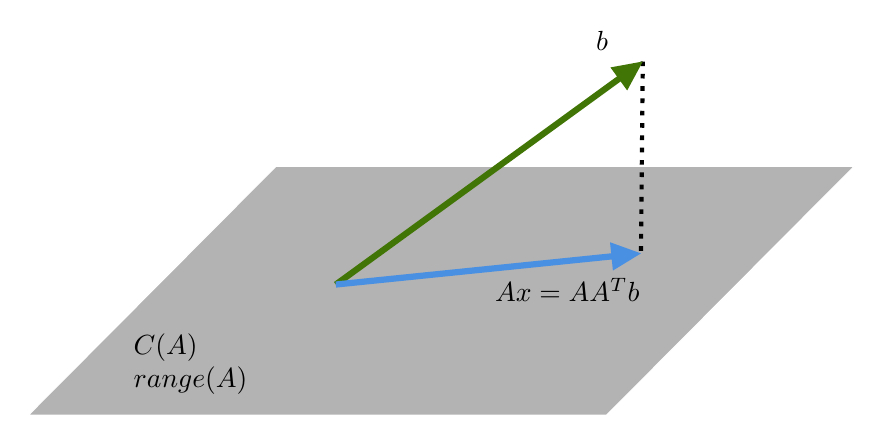
\begin{tikzpicture}[x=0.75pt,y=0.75pt,yscale=-1,xscale=1]
%uncomment if require: \path (0,300); %set diagram left start at 0, and has height of 300

%Shape: Parallelogram [id:dp5765772576295551] 
\draw  [color={rgb, 255:red, 255; green, 255; blue, 255 }  ,draw opacity=1 ][fill={rgb, 255:red, 179; green, 179; blue, 179 }  ,fill opacity=1 ] (203.26,170) -- (481.86,170) -- (362.46,290) -- (83.86,290) -- cycle ;
%Straight Lines [id:da4794253301098559] 
\draw [color={rgb, 255:red, 0; green, 0; blue, 0 }  ,draw opacity=1 ][line width=1.5]  [dash pattern={on 1.69pt off 2.76pt}]  (379.96,119.55) -- (379.07,212) ;
%Straight Lines [id:da5251055282063475] 
\draw [color={rgb, 255:red, 65; green, 117; blue, 5 }  ,draw opacity=1 ][line width=2.25]    (232.07,227) -- (375.92,122.49) ;
\draw [shift={(379.96,119.55)}, rotate = 504] [fill={rgb, 255:red, 65; green, 117; blue, 5 }  ,fill opacity=1 ][line width=0.08]  [draw opacity=0] (14.29,-6.86) -- (0,0) -- (14.29,6.86) -- cycle    ;
%Straight Lines [id:da14492521891839827] 
\draw [color={rgb, 255:red, 74; green, 144; blue, 226 }  ,draw opacity=1 ][line width=2.25]    (232.07,227) -- (374.09,212.51) ;
\draw [shift={(379.07,212)}, rotate = 534.1700000000001] [fill={rgb, 255:red, 74; green, 144; blue, 226 }  ,fill opacity=1 ][line width=0.08]  [draw opacity=0] (14.29,-6.86) -- (0,0) -- (14.29,6.86) -- cycle    ;

% Text Node
\draw (126.72,248.11) node [anchor=north west][inner sep=0.75pt]    {$ \begin{array}{l}
C( A)\\
\operatorname{range}( A)
\end{array}$};
% Text Node
\draw (356.21,103.52) node [anchor=north west][inner sep=0.75pt]    {$b$};
% Text Node
\draw (307.57,222.9) node [anchor=north west][inner sep=0.75pt]    {$Ax=AA^{T} b$};


\end{tikzpicture}

\end{FigureCenter}


\begin{problem}
    假设矩阵 $ A \in \mathbb{R}^{m \times n} $ \textbf{具有标准正交列},求投影$b$在$C(A)$上的投影。
\end{problem}

即向量 $ A x $ 与$b$有最短距离

$$
\min _{x}\|A x-b\|_{2}^{2}
$$

$$ \begin{aligned} f(x) &=\|A x-b\|_{2}^{2}
    \\ & =(A x-b)^{T}(A x-b)=x^{T} A^{T} A x-2 x^{T} A^{T} b+b^{T} b \\ &=x^{T} x-2 x^{T} A^{T} b+b^{T} b\left(\because A^{T} A=I\right) \end{aligned} $$

$$ \nabla f(x)=2 x-2 A^{T} b=0 \Rightarrow x=A^{T} b $$

$ A A^{T} b $ 称为向量 $  {b} \in \mathbb{R}^{m} $ 在 $ \operatorname{range} (A)$上的\term{正交投影}.

\begin{theorem}
    $$ A x=A A^{T} b \in \operatorname{range}(A) $$

    且是$b$在$C(A)$上的\term{投影}.
\end{theorem}

\begin{proof}
    1.
    $$ A x=A A^{T} b \in \operatorname{range}(A) $$

    2. 可以证明$ \hat{x}=A^{T} b $ 满足 $ \|A \hat{x}-b\|<\|A x-b\| $, 对于所有 $ x \neq \hat{x} $.

    b到range(A)内任意点 $ A x $ 的距离的平方和为:

    $$ \begin{aligned}\|A x-b\|_{2}^{2} &=\|A(x-\hat{x})+A \hat{x}-b\|_{2}^{2} \quad\left(\text {其中 } \hat{x}=A^{T} b\right) \\ &=\|A(x-\hat{x})\|_{2}^{2}+\|A \hat{x}-b\|_{2}^{2}+2(x-\hat{x})^{T} A^{T}(A \hat{x}-b) \\ &=\|A(x-\hat{x})\|_{2}^{2}+\|A \hat{x}-b\|_{2}^{2} \\ &=\|(x-\hat{x})\|_{2}^{2}+\|A \hat{x}-b\|_{2}^{2} \\ & \geq\|A \hat{x}-b\|_{2}^{2} \end{aligned} $$
当且仅当 $ x=\hat{x} $, 等号成立。

第3行成立是因为 $ A^{T}(A \hat{x}-b)=\hat{x}-A^{T} b=0 $ .
\end{proof}

\begin{FigureCenter}{Projection of $\boldsymbol{b}$ into the column space of ${A}$, $A$ is any matrice. Sourced from \cite{Strang1993IntroductionTL}}
    \tikzset{every picture/.style={line width=0.75pt}} %set default line width to 0.75pt        

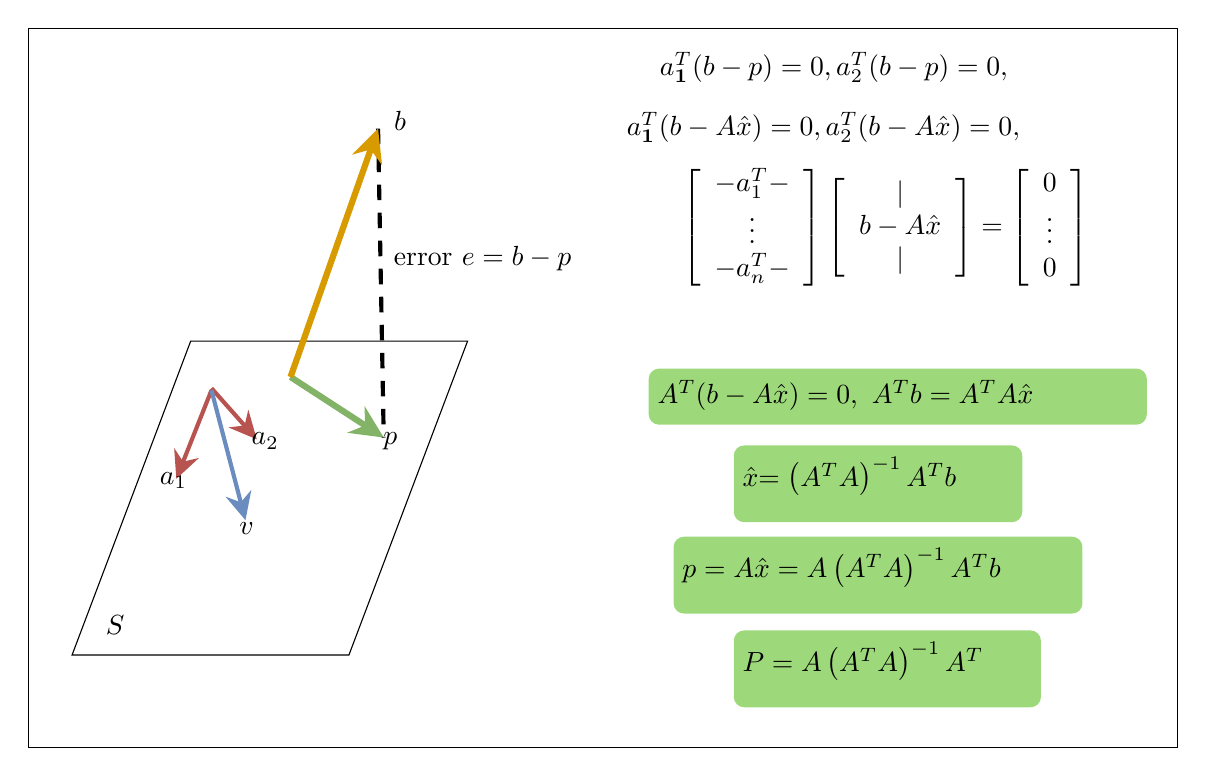
\begin{tikzpicture}[x=0.75pt,y=0.75pt,yscale=-1,xscale=1]
%uncomment if require: \path (0,350); %set diagram left start at 0, and has height of 350

%Straight Lines [id:da0833896477217686] 
\draw [color={rgb, 255:red, 130; green, 179; blue, 102 }  ,draw opacity=1 ][line width=2.25]    (127.38,169.03) -- (168.08,195.47) ;
\draw [shift={(172.28,198.19)}, rotate = 213] [fill={rgb, 255:red, 130; green, 179; blue, 102 }  ,fill opacity=1 ][line width=0.08]  [draw opacity=0] (16.07,-7.72) -- (0,0) -- (16.07,7.72) -- (10.67,0) -- cycle    ;
%Straight Lines [id:da7639150841734914] 
\draw [color={rgb, 255:red, 184; green, 84; blue, 80 }  ,draw opacity=1 ][line width=1.5]    (89.28,175.43) -- (73.82,214.38) ;
\draw [shift={(72.35,218.1)}, rotate = 291.64] [fill={rgb, 255:red, 184; green, 84; blue, 80 }  ,fill opacity=1 ][line width=0.08]  [draw opacity=0] (13.4,-6.43) -- (0,0) -- (13.4,6.44) -- (8.9,0) -- cycle    ;
%Straight Lines [id:da3617082286190523] 
\draw [line width=1.5]  [dash pattern={on 5.63pt off 4.5pt}]  (169.55,49.34) -- (172.28,198.19) ;
%Shape: Parallelogram [id:dp7592583426452624] 
\draw   (79.28,151.73) -- (212.68,151.73) -- (155.51,303) -- (22.11,303) -- cycle ;
%Straight Lines [id:da8449665178781662] 
\draw [color={rgb, 255:red, 184; green, 84; blue, 80 }  ,draw opacity=1 ][line width=1.5]    (89.28,174.43) -- (108.47,196.09) ;
\draw [shift={(111.12,199.08)}, rotate = 228.46] [fill={rgb, 255:red, 184; green, 84; blue, 80 }  ,fill opacity=1 ][line width=0.08]  [draw opacity=0] (13.4,-6.43) -- (0,0) -- (13.4,6.44) -- (8.9,0) -- cycle    ;
%Straight Lines [id:da21760172692551993] 
\draw [color={rgb, 255:red, 106; green, 140; blue, 190 }  ,draw opacity=1 ][line width=1.5]    (89.28,175.43) -- (104.64,234.14) ;
\draw [shift={(105.66,238.01)}, rotate = 255.32999999999998] [fill={rgb, 255:red, 106; green, 140; blue, 190 }  ,fill opacity=1 ][line width=0.08]  [draw opacity=0] (13.4,-6.43) -- (0,0) -- (13.4,6.44) -- (8.9,0) -- cycle    ;
%Straight Lines [id:da9743594112783229] 
\draw [color={rgb, 255:red, 215; green, 155; blue, 0 }  ,draw opacity=1 ][line width=2.25]    (127.38,169.03) -- (167.89,54.06) ;
\draw [shift={(169.55,49.34)}, rotate = 469.41] [fill={rgb, 255:red, 215; green, 155; blue, 0 }  ,fill opacity=1 ][line width=0.08]  [draw opacity=0] (16.07,-7.72) -- (0,0) -- (16.07,7.72) -- (10.67,0) -- cycle    ;
%Shape: Rectangle [id:dp3830905409317218] 
\draw   (1,1) -- (554.64,1) -- (554.64,347.62) -- (1,347.62) -- cycle ;

% Text Node
\draw (175.98,39.87) node [anchor=north west][inner sep=0.75pt]    {$\boldsymbol{b}$};
% Text Node
\draw (170.85,194.49) node [anchor=north west][inner sep=0.75pt]    {$\boldsymbol{p}$};
% Text Node
\draw (107.38,194.77) node [anchor=north west][inner sep=0.75pt]    {$\boldsymbol{a}_{2}$};
% Text Node
\draw (175.92,104.86) node [anchor=north west][inner sep=0.75pt]   [align=left] {error $\displaystyle \boldsymbol{e} =\boldsymbol{b-p}$};
% Text Node
\draw (63.21,213.92) node [anchor=north west][inner sep=0.75pt]    {$\boldsymbol{a}_{1}$};
% Text Node
\draw (101.48,237.88) node [anchor=north west][inner sep=0.75pt]    {$\boldsymbol{v}$};
% Text Node
\draw (37.18,282.9) node [anchor=north west][inner sep=0.75pt]    {$\boldsymbol{S}$};
% Text Node
\draw (288.11,40.4) node [anchor=north west][inner sep=0.75pt]    {$\boldsymbol{a}_{\mathbf{1}}^{T} (\boldsymbol{b} -\boldsymbol{A}\hat{\boldsymbol{x}} )=0,\boldsymbol{a}_{2}^{T} (\boldsymbol{b} -\boldsymbol{A}\hat{\boldsymbol{x}} )=0,\dotsc $};
% Text Node
\draw (304.11,11.4) node [anchor=north west][inner sep=0.75pt]    {$\boldsymbol{a}_{\mathbf{1}}^{T} (\boldsymbol{b} -\boldsymbol{p} )=0,\boldsymbol{a}_{2}^{T} (\boldsymbol{b} -\boldsymbol{p} )=0,\dotsc $};
% Text Node
\draw (314.93,67.4) node [anchor=north west][inner sep=0.75pt]    {$\left[\begin{array}{ c }
-\boldsymbol{a}_{1}^{{T}} -\\
\vdots \\
-\boldsymbol{a}_{n}^{{T}} -
\end{array}\right]\left[\begin{array}{ c }
\mid \\
\boldsymbol{b} -\boldsymbol{A\hat{\boldsymbol{x}}}\\
\mid 
\end{array}\right] =\left[\begin{array}{ c }
0\\
\vdots \\
0
\end{array}\right]$};
% Text Node
\draw  [color={rgb, 255:red, 0; green, 0; blue, 0 }  ,draw opacity=0 ][fill={rgb, 255:red, 157; green, 217; blue, 123 }  ,fill opacity=1 ]  (299.93,170) .. controls (299.93,167.24) and (302.17,165) .. (304.93,165) -- (534.93,165) .. controls (537.7,165) and (539.93,167.24) .. (539.93,170) -- (539.93,187) .. controls (539.93,189.76) and (537.7,192) .. (534.93,192) -- (304.93,192) .. controls (302.17,192) and (299.93,189.76) .. (299.93,187) -- cycle  ;
\draw (302.93,169.4) node [anchor=north west][inner sep=0.75pt]    {$\boldsymbol{A^{T} (b-A\hat{x} )} =0,\ \boldsymbol{A^{T} b=A^{T} A\hat{x}}$};
% Text Node
\draw  [color={rgb, 255:red, 0; green, 0; blue, 0 }  ,draw opacity=0 ][fill={rgb, 255:red, 157; green, 217; blue, 123 }  ,fill opacity=1 ]  (340.93,207) .. controls (340.93,204.24) and (343.17,202) .. (345.93,202) -- (474.93,202) .. controls (477.7,202) and (479.93,204.24) .. (479.93,207) -- (479.93,234) .. controls (479.93,236.76) and (477.7,239) .. (474.93,239) -- (345.93,239) .. controls (343.17,239) and (340.93,236.76) .. (340.93,234) -- cycle  ;
\draw (343.93,206.4) node [anchor=north west][inner sep=0.75pt]    {$\hat{\boldsymbol{x}}\boldsymbol{=\left( A^{T} A\right)^{-1} A^{T} b}$};
% Text Node
\draw  [color={rgb, 255:red, 157; green, 217; blue, 123 }  ,draw opacity=0 ][fill={rgb, 255:red, 157; green, 217; blue, 123 }  ,fill opacity=1 ]  (311.93,251) .. controls (311.93,248.24) and (314.17,246) .. (316.93,246) -- (503.93,246) .. controls (506.7,246) and (508.93,248.24) .. (508.93,251) -- (508.93,278) .. controls (508.93,280.76) and (506.7,283) .. (503.93,283) -- (316.93,283) .. controls (314.17,283) and (311.93,280.76) .. (311.93,278) -- cycle  ;
\draw (314.93,250.4) node [anchor=north west][inner sep=0.75pt]    {$\boldsymbol{p=A\hat{x} =A\left( A^{T} A\right)^{-1} A^{T} b}$};
% Text Node
\draw  [color={rgb, 255:red, 0; green, 0; blue, 0 }  ,draw opacity=0 ][fill={rgb, 255:red, 157; green, 217; blue, 123 }  ,fill opacity=1 ]  (340.93,296.15) .. controls (340.93,293.38) and (343.17,291.15) .. (345.93,291.15) -- (483.93,291.15) .. controls (486.7,291.15) and (488.93,293.38) .. (488.93,296.15) -- (488.93,323.15) .. controls (488.93,325.91) and (486.7,328.15) .. (483.93,328.15) -- (345.93,328.15) .. controls (343.17,328.15) and (340.93,325.91) .. (340.93,323.15) -- cycle  ;
\draw (343.93,295.55) node [anchor=north west][inner sep=0.75pt]    {$\boldsymbol{P=A\left( A^{T} A\right)^{-1} A^{T}}$};


\end{tikzpicture}

\end{FigureCenter}


    
